%\documentstyle{article}  % by default 10pt
\documentclass{article}  % by default 10pt

\usepackage{graphicx}
\usepackage{amsfonts}
\usepackage{subfigure}
\usepackage{times}
\usepackage{cite}
\usepackage{subfigure}
\usepackage{amsmath}
\usepackage{amssymb}
\usepackage{url}
\usepackage{tikz}
\usepackage{verbatim}
\usepackage{array}
\usepackage{wrapfig}

%
% Page dimensions.
%
\oddsidemargin  -0.2in % 
\evensidemargin -0.2in %
\topmargin      -1.00in % (adjusted for printer bias)
\headheight      .00in  % (no headers)
\headsep         .75in  % (top margin + headers + skip)
%\footheight     12.0pt  % ??? (seems to work ok)
\footskip       75.0pt  % ??? ( "   "  )
\textheight     9.425in % (instructions: 9 1/8" min, 9 7/16" max)
\textwidth      6.7in   %
%\linespread{0.9}
%
  % Paragraph changes.
  %

  \parindent=10pt
  %\parskip=10pt
  %


  \def\@maketitle{\vbox to 2.6in{\hsize\textwidth
    \linewidth\hsize \vfil \centering
    {\large \@title \par}
    \vskip 2em
    {\normalsize
      \begin{tabular}[t]{c}\@author
	\end{tabular}\par}
      \vfil}
  }


\begin{document}

%\title{Integrated Modeling of Performance, Power and Resilience for Adaptive Parallelism}
\title{\emph{Adaptive Parallelism}: Integrated Performance, \\Power, and Resilience Modeling}


\author{Dong Li$^{\dag}$, Edgar A. Le{\'o}n$^{\star}$, and Bronis R. de Supinski$^{\star}$ \\
    $^{\dag}$Oak Ridge National Laboratory and $^{\star}$Lawrence Livermore National Laboratory \\
    lid1@ornl.gov (main contact), \{leon,bronis\}@llnl.gov	\\
}

\date{}

\maketitle

\noindent {\Large \textbf{The Need for Integrated Modeling}}\\
From embedded devices to future exascale computers, increased
parallelism in both the number of processing units and nodes will
create unprecedented challenges to achieve the expected levels of
application performance. System power consumption will be a major 
consideration. For large-scale systems, failures proportional
to the size of the system will impair system usability. To address 
these challenges, modeling methods must evolve and consider the 
combined effects of performance, power, and resilience (PPR). 
Further, modeling methods must be rapid and accurate to evaluate 
the dynamic tradeoffs posed by PPR in large-scale systems. 

% The path to exascale presents increased parallelism to reach performance targets with constrained power consumption.
% Meanwhile, efforts to reduce power and increase component counts may lead to significant increase in the number of faults,
% making system resilience a grand challenge for exascale systems.
% To address challenges of performance, power, and resilience (PPR),
% modeling methods must evolve and consider them in
% concert. Furthermore, modeling methods must be rapid and accurate,
% such that runtime can effectively enable dynamic evaluation of
% tradeoffs between PPR. 

Many current modeling methods employ analytical models or architectural, 
highly-accurate simulators. Analytical models tend to focus on a specific 
dimension of performance, power, and resilience but often miss the combined 
interdependent effects. Highly accurate simulators, on the other hand, are 
not scalable. Further, the overhead imposed by many modeling tools is too 
high to be used at runtime. Thus, we need more efficient and unified modeling
frameworks, which will enable runtime systems to find, in real-time, an
efficient operating point in terms of PPR for an application. 


% The common practice of current modeling methods employs analytical models or architectural simulators to study PPR.
% The investigations of performance, power, and resilience are isolated based on individual modeling infrastructures
% and methodologies.
% Furthermore, many modeling tools and techniques are heavyweight, and cannot be easily employed at runtime.
% As a result, we do not have any efficient modeling mechanism that directs runtime management 
% and allows us to explore the optimal operating point in the 3D search space of PPR.

In this paper, we propose an infrastructure for modeling parallelism
and its combined effects on performance, power, and resilience. Managing 
and optimizing parallelism dynamically is at the core of meeting the 
challenging requirements of PPR imposed by future systems. The inherent 
parallelism of scientific applications varies across execution 
phases~\cite{nvram_ipdps12}.  Matching the degree of parallelism 
(\textit{parallel configuration}) for an application has complex PPR 
implications~\cite{mpiopenmp_ipdps10, mpiopenmp_tpds13, dsn_pact08, dsn_ics06}.
Our goal is to develop a model-driven approach based on hardware resource 
utilization that will guide the selection and adaptation of parallel 
configurations.


%  We collect resource utilization information from  
% a common set of hardware components to characterize applications and
% predict PPR. 

% We study our modeling techniques in the context of runtime parallelism management for the OpenMP
% programming model.


% In this paper, we propose modeling of PPR based on an integrated %uniform 
% modeling infrastructure. 
% The infrastructure collects utilization information from 
% a common set of hardware components to characterize applications and predict PPR.
% We study our modeling techniques in the context of runtime parallelism management for the OpenMP
% programming model.
% The management and optimization of parallelism is fundamental to meet PPR requirements
% of exascale systems.
% Scientific applications typically have inherent parallelism that varies across execution phases~\cite{nvram_ipdps12}.
% Matching the degree of parallelism (named \textit{parallelism configuration} in the rest of paper) between application and hardware
% have complicated implications on PPR~\cite{mpiopenmp_ipdps10, mpiopenmp_tpds13, dsn_pact08, dsn_ics06}. 
% We aim to use a model-driven approach to decide optimal parallelism based on user-defined policies
% and enable adaptive parallelism at runtime.

%dynamic parallelism is at the core of PPR... 

%Relative order; no absoultely requirement on accuracy.
%The path to exascale presents increased parallelism with billions of concurrently-executing threads 
%at the intra-node and inter-node levels. 
%The management and optimization of parallelism is fundamental to meet performance, 
%energy-efficiency and resilience requirements
%of systems and applications at exascale.

\vspace{10pt}

\noindent {\Large \textbf{Adaptive Parallelism Framework}}  \\
We base our proposed modeling methodology on two observations.
First, performance, power, and resilience have first-order or
second-order correlations with hardware component utilization.
From a performance perspective, our work reveals, for example, that
the number of accesses to the memory hierarchy and the number of
executed instructions serve as strong indicators of performance with
various levels of 
parallelism~\cite{mpiopenmp_tpds13, mpiopenmp_ipdps10, dct_pmbs11, dct_iiswc12}. 
Power consumption is related to hardware usage 
intensity~\cite{leon:14:characterizing,mpiopenmp_tpds13, powermodel_sigmetrics03, powermodel_micro03}.
Resilience is related to both application execution time, $t$, and number of 
hardware accesses, $hwacc$. Given hardware failure rates for specific hardware
components, longer application execution times and more hardware accesses 
expose the application to more random occurrences of hardware failures 
(including both hard and soft errors). We introduce a new metric, the
\textit{vulnerability factor} (VF), which is defined as $VF = t*hwacc$, 
to quantify application vulnerability. Thus, resilience,
like performance and power, is related to hardware component utilization.

% EL: how about vf = sum over components {hwaccess(time) *
% component_failure_rate}? We don't need to explicitly state the
% formula but that vf is a function of execution time, hardware
% accesses driven by application characteristics, and component
% failure rate... 
 
Second, given a parallel region, PPR and thread-level parallelism are
strongly correlated  statistically. Thus, based on hardware components 
utilization collected from a few samples of parallel configurations, 
%(each of which employs a specific number of OpenMP threads),  
we can predict PPR for other parallel configurations. 
We call these representative samples \textit{seminal configurations}.

Based on these observations, we can construct an integrated, PPR model 
in two phases: offline model training and online model selection. Model 
training uses machine learning to determine the hardware component 
utilization information that is most correlated with PPR. The information 
should be measurable with lightweight hardware counters. Also, seminal 
configurations are chosen empirically. Empirical observations reveal that 
PPR data with different levels of parallelism can be clustered into different 
groups. The parallel configuration that is the \emph{closest} to the center 
of each group is chosen as a seminal configuration. 
% EL: we need to explain what we mean by "closest"
During offline training, we build a series of PPR models to capture diverse 
hardware features and application characteristics. Using a diverse set of 
applications and benchmarks during training is key to producing accurate 
models. During online model selection, we use a few sample iterations of
parallel regions to execute with seminal configurations and collect
hardware component utilization information in order to identify the model 
to use.

Based on the above modeling methodology, we can accurately predict PPR
at runtime for any untested parallelism configuration with low
overhead. We enable accurate on-line modeling by building the model offline 
using a diverse set of application characteristics. Using the resulting models,
a runtime system can use high-level policies that indicate the desired levels
of performance, power, and resilience. For example, minimizing the
vulnerability factor at a marginal performance and power cost; and
achieving the best performance and resilience within a power
cap. Figure~\ref{fig:general_framework} provides an overview of our 
framework's model construction and deployment.

% Built on top of the models,
% runtime chooses the best parallelism for each OpenMP parallel region based 
% on high-level user-defined policies, for example, minimizing VF without performance and power
% loss, or minimizing the multiplication of time, power, and VF to achieve
% an optimal tradeoff of PPR, or achieving the best performance and
% resilience within a power cap.
Our previous investigations show that this methodology can
predict performance and power with high accuracy on many-core
platforms. These results are encouraging and we plan to integrate our
proposed resiliency model into this framework. Looking forward, future
milestones include the creation of models for emerging heterogenous
memory architectures (multiple levels of memory to provide bandwidth
and capacity requirements of future systems), analyzing the effects of
data layout and memory parallelism on PPR, and developing new models
for heterogenous computing platforms.
%% BRONIS: The following seems random since we have not discussed
%% BRONIS: OpenMP prior to this statement.
%% We will leverage our OpenMP expertise to implement our proposed infrastructure. 

% We have established the model infrastructure to predict performance and power on many-core platforms.
% We plan to extend the modeling methodology to better capture effects of
% data layout and memory-level parallelism on PPR.
% We also plan to extend the models to support PPR prediction 
% and parallelism scheduling on
% heteroegenous platforms. 
%to be a new layer between OpenMP directives,

\begin{wrapfigure}{r}{0.4\textwidth}
\begin{center}
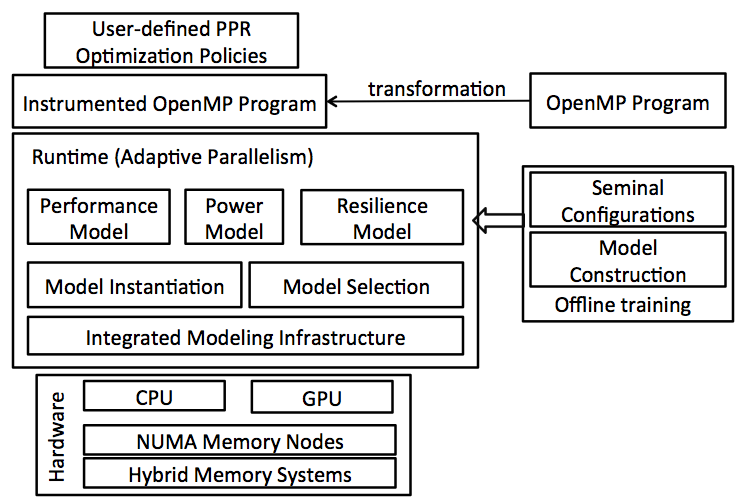
\includegraphics[width=0.39\textwidth]{figures/general_framework.png}
\end{center}
\caption{The general framework for adaptive parallelism with integrated PPR modeling}
\label{fig:general_framework}
\end{wrapfigure}

\vspace{10pt}

\noindent {\Large \textbf{Related Work}}   \\
Performance, power, and resilience modeling and simulation have been
studied before, but mostly in isolation. Some related work employs
analytical or empirical models to achieve joint optimization of power
and performance. For example, Green 
Queue~\cite{sdscpower_hppac12, sdscpower_ccpe12, sdscpower_cgc12},  
Adagio~\cite{rountree_sc07, rountree_ics09}, and Workload
Consolidation~\cite{taskconsolidation_ipdps10,   gpusolidation_srmpds11}. 
Other work uses detailed hardware analysis for hardware-oriented resilience 
modeling. For example, Mukherjee et al.~\cite{avf_micro03} define 
architectural vulnerability factor (AVF) as the probability that a
fault in a particular structure will result an error. 
Biswas et al.~\cite{avf_isca05} show how to compute the AVF of address-based
processor structures based on a detailed analysis of architecturally
correct execution. Sridharan and Kaeli~\cite{pvf_selse10, pvf_hpca09}
introduce a new metric to capture the architecture-level fault masking
inherent in a program. In addition, fault injection has been
widely used to understand application 
vulnerability~\cite{li:2012:classifying, multigrid_ics12, fj_asplos12, fj_dns12, lanl_fi_europar11}.

\vspace{10pt}

%Challenges addressed: Which modeling and/or simulation challenges
%does this approach address? 
\noindent {\Large \textbf{Evaluation of Proposed Methodology}}   \\
\textbf{Challenges}. 
Future systems demand modeling and simulation capabilities to help us
understand the complex and combined interactions between performance,
power, and resilience. Further, modeling and simulation techniques
should provide rapid and dynamic evaluation of tradeoffs between
them. Our proposed modeling infrastructure is designed to provide
lightweight and accurate PPR predictions based on adaptive
parallelism. It can be used by runtime systems to manage system
resources for a specific set of objectives based on thread-level and
memory-level parallelism.  

%extremely
%valuable for runtime management of system resource (e.g., thread-level parallelism and  
%memory-level parallelism in our case).
%The proposed approach addresses resilience and power challenges for future exascale systems as

%Maturity: What are the indicators that this approach will address the
%identified challenges? 
\noindent\textbf{Maturity}. 
Our previous investigations show that our
proposed methodology can provide accurate and lightweight modeling 
of performance and power for OpenMP parallel regions on several
multicore architectures~\cite{mpiopenmp_ipdps10, mpiopenmp_tpds13,
  taskconsolidation_ipdps10, dct_iiswc12, dct_pmbs11}. We have
successfully applied  
machine-learning techniques to this area to address the challenges
associated with an extremely large space of optimizations. This 
infrastructure provides a strong basis for integrating
modeling of different objective functions. Adding modeling
capabilities for resilience and reliability along with processor and
memory heterogeneity will undoubtedly present significant challenges. 

% Performance, power and resilience modeling and simulation have been separatrely considered in the
% existing work (see related work).
% Also, we have established preliminary capabilities to model performance and power for OpenMP parallel 
% regions with various parallel configurations. Our modeling infrastructure brings ignorable 
% performance overhead while providing great energy saving for DOE applications with 
% the hybrid MPI/OpenMP programming model.
% However, our current modeling infrastructure is only a start and
% requires significant new work to improve modeling infrastructure
% especially for resilience modeling and heterogeneous platform. 
%The proposed idea builds on successful research, including the DOE funded Blackcomb 

%Uniqueness: To what extent is the proposed approach unique? Could it
%be addressed by other research programs? 
\noindent\textbf{Uniqueness}.
A key feature of our modeling methodology is our focus on
parallelism, which is the central consideration in managing the tradeoffs
between power, performance, and resilience. In addition, we will use
machine-learning techniques to create multi-dimensional PPR models.
The goal of our modeling infrastructure is to guide a runtime system 
to determine the \emph{right} level of concurrency to achieve desired 
optimization objectives. 

% Our modeling methodology is tightly coupled with the OpenMP programming model,
% and aims to reveal PPR difference between different parallelism configurations.
% Unlike prior work that focuses on accurate prediction, our work
% focuses on coarse-grained PPR indicator to guide runtime management. 

%Novelty: How is this approach different from existing solutions?
\noindent\textbf{Novelty}. 
Our modeling methodology reveals statistical correlation
between measurable hardware events, application characteristics, and 
PPR. The unique set of features and opportunities provided by our models
provide fast exploration of PPR to achieve multi-dimensional optimization.     

%Applicability: To what extent will the proposed approach, if
%successful, be applicable to other areas? 
\noindent\textbf{Applicability}. 
The proposed PPR models have been deployed in an OpenMP runtime to
optimize performance and energy efficiency by using adaptive
parallelism. Our thesis is that this approach can be successfully applied
to other areas such as modeling of emerging memory systems. 

% The proposed models work
% as a critical step to implement adaptive parallelism, 
% and provide a new approach for massive parallelism management.

%Effort: How much effort is needed to effectively explore this approach?
\noindent\textbf{Effort}. 
Key milestones include developing models of resilience and memory-level 
parallelism and investigating their interactions with other 
objectives such as power and performance. In addition, we need to
investigate the accuracy and overhead of our modeling methodology on a
variety of hardware  resources including homogenous and heterogenous
processor architectures, and emerging heterogeneous memory architectures
(multi-level memories). 

% We need to add new features into the current modeling infrastructure,
% including resilience modeling and memory-level parallelism modeling,
% and interoperating with other ModSim tools.
% To provide a broad coverage of system properties and resources, we need
% a significant effort contributing to an agile and integrated modeling
% of PPR.

\bibliography{li}
\bibliographystyle{plain}

\end{document}
